\chapter{Algèbre linéaire, Matrices}
\labch{algebre_lineaire_matrices}

\textsl{Au \textsc{xviii}$^\me$ siècle se développent la résolution des systèmes linéaires et la théorie des déterminants. Les raisonnements suggèrent rapidement le concept d'espace à $n$ dimensions. Mais il fallait oser un langage géométrique, alors qu'une interprétation sensible dans le plan ou l'espace faisait défaut pour $n > 3$. \\
De manière indépendante, \textsc{Cayley} en Angleterre et \textsc{Grassman} en Allemagne franchissent le pas vers 1843-1845 et parlent d'espace à $n$ dimensions. Le point de vue de \textsc{Cayley} est issu directement de la géométrie analytique: un vecteur d'un espace à $n$ dimensions est un système de $n$ réels ou $n$ complexes. L'addition de deux vecteurs et la multiplication par un scalaire sont naturellement introduites par la généralisation de la dimension $3$. Pour parvenir vraiment à la notion d'espace vectoriel, il faut dégager le concept de sous-espace et de dimension d'un sous-espace. C'est ce que fera \textsc{Grassman} (professeur de lycée autodidacte en marge des milieux de la recherche) en cherchant à développer une analyse géométrique portant sur des calculs intrinsèques indépendants du choix des coordonnées. \textsc{Grassman} introduit le produit extérieur de deux vecteurs, la définition de l'indépendance linéaire, de la dimension d'un espace et démontre la relation fondementale
$$\dim V + \dim W = \dim (V + W) + \dim V \cap W.$$
Ces travaux eurent peu d'impact au début, mais ils furent repris par Henri \textsc{Poincaré} et Élie \textsc{Cartan} (notamment son \say{algèbre extérieure} en géométrie différentielle). \\
C'est en 1888 que \textsc{Peano} donnera la définition axiomatique d'un espace vectoriel réel. Jusqu'en 1930, le point de vue des matrices et des coordonnées prédomine par rapport au point de vue intrinsèque des espaces vectoriels.
}

\begin{marginfigure}[-13cm]
    \centering
    \includegraphics{images/arthur_cayley.png}
    \caption*{\centering Arthur \textsc{Cayley} (1821-1895)}
\end{marginfigure}

\begin{marginfigure}[-6cm]
    \centering
    \includegraphics{images/hermann_grassmann.png}
    \caption*{\centering Hermann \textsc{Grassmann} (1809-1877)}
\end{marginfigure}

\newpage

% \section{Cours: changement de base}
% \begin{marginfigure}
%     \tikzset{>=latex} % for LaTeX arrow head
\colorlet{xcol}{blue!70!black}
\tikzstyle{rvec}=[->,thick,xcol,line cap=round]

% VECTOR breakdown on axis
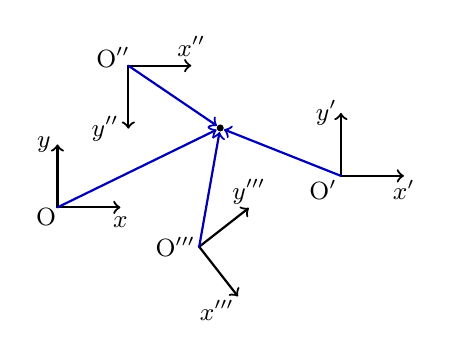
\begin{tikzpicture}
  \small
  \def\L{0.8}
  \def\R{2.3}
  \def\ang{26}
  \def\thet{-52}
  \coordinate (O) at (0,0);
  \coordinate (O1) at (3.6,0.4);
  \coordinate (O2) at (0.9,1.8);
  \coordinate (O3) at (1.8,-0.5);
  \coordinate (R) at (\ang:\R);
  \node[fill=black,circle,inner sep=0.9] (R') at (R) {};
  
  % O1
  \draw[<->,thick] (\L,0) node[below] {$x$} --
                   (O) node[below left=-3] {O} --
                   (0,\L) node[left=-1] {$y$};
  \draw[rvec] (O) -- (R');
  
  % O1
  \begin{scope}[shift={(O1)}]
    \draw[<->,thick] (\L,0) node[below=-2] {$x'$} --
                     (0,0) node[below left=-2] {O$'$} --
                     (0,\L) node[left=-2] {$y'$};
    \draw[rvec] (0,0) -- (R');
  \end{scope}
  
  % O2
  \begin{scope}[shift={(O2)}]
    \draw[<->,thick] (\L,0) node[above] {$x''$} --
                     (0,0) node[above left=-4] {O$''$} --
                     (0,-\L) node[left] {$y''$};
    \draw[rvec] (0,0) -- (R');
  \end{scope}
  
  % O3
  \begin{scope}[shift={(O3)}]
    \draw[<->,thick] (\thet:\L) node[below left=-2] {$x'''$} --
                     (0,0) node[left=-2] {O$'''$} --
                     (\thet+90:\L) node[above=-2] {$y'''$};
    \draw[rvec] (0,0) -- (R');
  \end{scope}
  
\end{tikzpicture}
% \end{marginfigure}

% \section{Produit d'endomorphismes nilpotents qui commutent}
% \begin{itemize}
    \item Lemme à démontrer: \\
    si $u$ et $v$ sont deux endomorphismes qui commutent, $v$ étant nilpotent, alors soit $u=0$ soit $\Rg(uv) < \Rg(u)$.\\
    \textcolor{green}{Revoir la démonstration}
\end{itemize}

\section{Centre de \texorpdfstring{$\M_n(\K)$}{l'espace des matrices carrées}}
\begin{defi}{Centre (algèbre)}
    Le \emph{centre} d'une structure algébrique est l'ensemble des éléments de cette structure qui commutent avec tous les autres éléments. 
\end{defi}

\begin{prop}{Centre de $\M_n(\K)$}
Le centre de $\M_n(\K)$, c'est-à-dire les matrices $A \in \M_n(\K)$ telles que pour toute matrice $B \in \M_n(\K), AB = BA$, est égal à l'ensemble des matrices scalaires.
\end{prop}

Nous voulons démontrer l'égalité de deux ensembles à savoir le centre de $\M_n(\K)$ et $\{ \lambda \I_n, \lambda \in \K \}$. Nous allons donc raisonner par double inclusion. 
\begin{preuve}
    \begin{itemize}
        \item[$(\subset)$] Posons $A \defeq (a_{i,j})_{1 \leqslant 1, j \leqslant n}$. Si la matrice $A$ appartient au centre de $\M_n(\K)$ alors, en particulier, elle commute avec les matrices élémentaires \note i.e. 
        \marginnote[0cm]{
            \begin{kaobox}[frametitle=\note Matrices élémentaires de $\M_{n,p}(\K)$]
                Pour tout $(i, j) \in \llbracket 1, n \rrbracket \times \llbracket 1, p \rrbracket$, on note $\mathrm{E}_{i,j}$ la matrice de taille $(n,p)$ dont tous les coefficients son nuls sauf le coefficient en ligne $i$, colonne $j$, qui est égal à $1$. Autrement dit,
                $$\mathrm{E}_{i,j} = (\delta_{k,i} \times \delta_{\ell, j})_{(k,\ell) \in \llbracket 1, n \rrbracket \times \llbracket 1, p \rrbracket}.$$
                On en déduit que 
                $$\mathrm{E}_{i,j} \times \mathrm{E}_{k, \ell} = \delta_{j,k} \mathrm{E}_{i, \ell}.$$
            \end{kaobox}
        }
        $$\forall (i, j) \in \llbracket 1, n \rrbracket^2, A \mathrm{E}_{i,j} = \mathrm{E}_{i,j} A.$$
        En décompasant la matrice $A$ dans la base des matrices élémentaires on obtient
        $$A \mathrm{E}_{i,j} = \sum_{1 \leqslant k, \ell \leqslant n} a_{k, \ell} \mathrm{E}_{k,\ell} \mathrm{E}_{i,j} = \sum_{k=1}^{n} a_{k,i} \mathrm{E}_{k,j},$$
        et
        $$\mathrm{E}_{i,j} A = \sum_{1 \leqslant k, \ell \leqslant n} a_{k, \ell} \mathrm{E}_{i,j} \mathrm{E}_{k,\ell} = \sum_{\ell=1}^{n} a_{j,\ell} \mathrm{E}_{i,\ell}.$$
        Puisque la famille $(\mathrm{E}_{i, j})_{1 \leqslant i, j \leqslant n}$ est libre, on peut identifier les coefficients des deux expressions et on déduit que pour tout $(i, k) \in \llbracket 1, n \rrbracket^2$ tel que $i \not= k, a_{i,k}=0$ et pour tout $(i,j) \in \llbracket 1, n \rrbracket^2, a_{i,i}=a_{j,j}$. \\
        Ainsi, si la matrice $A$ commute avec toutes les matrices, elle est nécessairement de la forme $A = \lambda \I_n$ où $\lambda \in \K$.
        \item[$(\supset)$] Réciproquement, pour tout $\lambda \in \K$ et toute matrice $B \in \M_n(\K), B \times (\lambda \I_n) = (\lambda \I_n) \times B$. 
    \end{itemize}
    On en déduit par double inclusion que le centre de $\M_n(\K)$ est égal à l'ensemble des matrices scalaires. 
\end{preuve}

\begin{methode}
    Lorsqu'il s'agit de montrer qu'une propriété est vraie \say{ pour toute matrice }, il est parfois utile de prendre des cas particuliers comme les \ptnclegras{matrices élémentaires} pour en déduire des informations sur les coefficients.
\end{methode}


\section{Semblables sur \texorpdfstring{$\C$, sur $\R$}{C, sur R}}
\begin{prop}{}
    Deux matrices réelles semblables dans $\M_n(\C)$ sont semblables dans $\M_n(\R)$.
\end{prop}

\begin{preuve}
    Soient $A$ et $B$ deux matrices réelles semblables dans $\M_n(\C)$. Alors il existe une matrice $P \defeq P_{\mathrm{r}} + \mi P_{\mathrm{i}} \in \Gl_n(\C)$ telle que $AP = PB$ soit $A P_{\mathrm{r}} + \mi A P_{\mathrm{i}} = P_{\mathrm{r}} B + \mi P_{\mathrm{i}} B$ et donc en identifiant parties réelle et imaginaire, $$A P_{\mathrm{r}} = P_{\mathrm{r}} B \text{ et } A P_{\mathrm{i}} = P_{\mathrm{i}} B.$$
    On en déduit que pour tout $x \in \R,\ A(P_{\mathrm{r}} + x P_{\mathrm{i}}) = (P_{\mathrm{r}} + x P_{\mathrm{i}})B$. On pose la fonction 
    $$\delta : z \in \C \mapsto \det(P_{\mathrm{r}} + z P_{\mathrm{i}}).$$ 
    La fonction $\delta$ est polynomiale et est non identiquement nulle car $\delta(\mi) = \det(P) \not=0$. On en déduit qu'il existe un réel $x_0$ tel que $\delta(x_0) = \det(P_{\mathrm{r}} + x_0 P_{\mathrm{i}}) \not=0$. \\
    Ainsi, en posant $\widetilde{P} \defeq P_{\mathrm{r}} + x_0 P_{\mathrm{i}} \in \Gl_n(\R)$ on obtient $A = \widetilde{P}B\Inv{\widetilde{P}}$.
\end{preuve}

\begin{remarque}
    Comme $\R \subset \C$, on en déduit que deux matrices sont semblables dans $\M_n(\C)$ si et seulement si elle le sont dans $\M_n(\R)$.
\end{remarque}

\begin{exercice}
    \marginnote[0cm]{Source : \cite{fmaalouf}}
    Soit $A \in \M_n(\R)$ telle que $\chi_A$ est scindé sur $\R$. Montrer que la matrice $A$ est diagonalisable dans $\M_n(\C)$ si et seulement si elle l'est dans $\M_n(\R)$.
\end{exercice}

\section{Noyaux itérés}
\begin{prop}{}
    Soit $E$ un espace vectoriel de dimension finie $n \in \Ne$. On considère $f \in \Endo(E)$.
    \begin{itemize}
        \item La suite $\left( \Ker(f^k) \right)_{k \in \N}$ est une suite croissante pour l'inclusion et stationnaire à partir d'un certain rang $r \in \llbracket 0, n \rrbracket$.
        \item La suite $\left( \Im(f^k) \right)_{k \in \N}$ est une suite décroissante pour l'inclusion et stationnaire à partir du même rang $r$. \\
        (la suite vient de \href{https://bibmath.net/dico/index.php?action=affiche&quoi=./n/noyauxiteres.html}{Noyaux itérés -- \textsf{Bibm@th.net}}) \\
        De plus
        $$\Ker(f^r) \oplus \Im(f^r) = E.$$
        Si on note $d_k \defeq \dim \big(\Ker(f^k) \big)$, alors pour tout $k \in \N$, 
        $$d_{k+1} - d_k \geqslant d_{k+2} - d_{k+1},$$
        autrement dit la suite de la différence des dimensions entre deux noyaux itérés consécutifs est décroissante. 
    \end{itemize}
\end{prop} 

Voir aussi énoncé de \cite{exos_oraux} p. 44.

\begin{demo}
    \begin{itemize}
        \item La monotonie des deux suites est triviale. 
        \item Bien précisier l'existe de $r$ en dimension finie. \\
        Soit $r$ le rang de stationnarité de la suite des noyaux itérés. Montrons que pour tout $k \in \N, \Ker(f^r) = \Ker(f^{r+k})$. \\
        D'après le premier item, l'une des deux inclusions est vérifiée par croissance de la suite des noyaux itérés. Montrons la deuxième. Soient $k \in \N$ et $x \in \Ker(f^{r+k+1})$. Alors $f^{r+k+1}(x) = f^{r+1} \big(f^k(x) \big) = 0$ soit $f^k(x) \in \Ker(f^{r+1}) = \Ker(f^r)$. Ainsi, $f^{r+k}(x) = 0$ et $x \in \Ker(f^{r+k})$.
        \item Montrons que $\Ker(f^r) \oplus \Im(f^r) = E$. \\
        D'après le théorème du rang, $\Rg(f^r) + \dim \Ker(f^r) = n$. Il reste à montrer que $\Ker(f^r) \cap \Im(f^r) = \{ 0 \}$. \\
        Soit $y \in \Ker(f^r) \cap \Im(f^r)$. Alors il existe $x \in E$ tel que $y = f^r(x)$. De plus, $f^r(y) = 0$ donc, en remplaçant $y$ par son expression, $f^{2r}(x) = 0$ i.e. $x \in \Ker(f^{2r})$, qui est égal à $\Ker(f^r)$ par définition de $r$. On en déduit que $y = f^r(x) = 0$. Ainsi $\Ker(f^r) \cap \Im(f^r) = \{ 0 \}$ et on a bien
        $$\Ker(f^r) \oplus \Im(f^r) = E.$$
    \end{itemize}
\end{demo}

\begin{remarque}
    La propriété de somme directe, n'est plus valable dans le cas d'un espace vectoriel de dimension infinie. En effet, dans $\R[X]$, l'application \emph{dérivée} met en défaut cette égalité. 
\end{remarque}

\begin{exercice}
    \marginnote[0cm]{Source : \cite{maths-france} Planche no 2. Révisions algèbre linéaire. Espaces vectoriels}
    Soient $E$ un espace vectoriel et $f$ un endomorphisme de $E$. Pour $k \in \N$, on pose $N_k \defeq \Ker(f^k)$ et $I_k \defeq \Im(f^k)$ puis $N \defeq \bigcup\limits_{k \in \N} N_k$ et $I \defeq \bigcap\limits_{k \in \N} I_k$. ($N$ est le nilespace de $f$ et $I$ le coeur de $f$).
    \begin{enumerate}
        \item 
        \begin{enumerate}
            \item Montrer que les suites $(N_k)_{k \in \N}$ et $(I_k)_{k \in \N}$ sont respectivement croissante et décroissante pour l'inclusion.
            \item Montrer que $N$ et $I$ sont stables par $f$. 
            \item Montrer que pour tout $k \in \N$, 
            $$(N_k = N_{k+1}) \implies (N_{k+1} = N_{k+2}).$$
        \end{enumerate}
        \item On suppose de plus que $\dim E = n$, $n \in \Ne$.
        \begin{enumerate}
            \item Soit 
            \begin{align*}
                A &\defeq \ens[\big]{ k \in \N \tq N_k = N_{k+1} } \\
                \text{et } B &\defeq \ens[\big]{k \in \N \tq I_k = I_{k+1}}.
            \end{align*}
            Montrer qu'il existe un entier $p$ inférieur à $n$ tel que $A = B =  \{ k \in \N \mid k \geqslant p \}$.
            \item Montrer que $E = N_p \oplus I_p$.
            \item Montrer que $f_{\vert N}$ est nilpotent et que $f_{\vert I} \in \Gl(I)$.
        \end{enumerate}
        \item Trouver des exemples où $A$ est vide et $B$ est non vide et où $A$ est non vide et $B$ est vide.
        \item Pour $k \in \N$, on pose $d_k \defeq \dim I_k$. Montrer que la suite $(d_k - d_{k+1})_{k \in \N}$ est décroissante. En déduire le sens de variation de la suite $\big( \dim N_{k+1} - \dim N_k \big)_{k \in \Ne}$.
    \end{enumerate}
\end{exercice}


\section{Applications de \texorpdfstring{$\M_n(\K) \to \K$}{l'espace des matrices carrées dans le corps K} conservant le produit}
\begin{defi}{Forme multiplicative}
    Soit $f$ une application de $\M_n(\K)$ dans $\K$. L'application $f$ est dite \emph{multiplicative} si pour tout matrices $A$ et $B$ de $\M_n(\K)$, $f(AB) = f(A)f(B)$.
\end{defi}

\begin{exercice}
    \marginnote[0cm]{\cite{exos_oraux} p. 53}
    Soit $n \in \Ne$ et $f$ une forme multiplicative de $\M_n(\K)$ dans $\K$ autre que les constantes $0$ et $1$. Montrer que $M \in \Gl_n(\K)$ si et seulement si $f(M) \not= 0$. 
\end{exercice}

\section{Matrices compagnon et commutant d'un cyclique}
\begin{defi}
    Soit $P(X) \defeq X^p + \sum\limits_{k=0}^{p-1} c_kX^k \in \K[X]$. On appelle \emph{matrice compagnon} de $P$ la matrice:
$$ C_P \defeq
\begin{pmatrix}
0 & 0 & \cdots & 0 & -c_0\\
1 & 0 & \cdots & 0 & -c_1\\
0 & 1 & \cdots & 0 & -c_2\\
\vdots & \vdots & \ddots & \vdots & \vdots\\
0 & 0 & \cdots & 1 & -c_{p-1}
\end{pmatrix}.
$$
\end{defi}

\begin{theo}
    Soit $P \in \K[X]$. Le polynôme $P$ est égal au polynôme caractéristique de sa matrice compagnon:
    $$\chi_{C_P}(X) = P(X).$$
\end{theo}   

\marginnote[2cm]{
    \begin{kaobox}[frametitle=Cofacteurs]
    \cite{acamanes} ch4
        Soient $A \in \M_n(\K)$ et $i, j \in \llbracket 1, n \rrbracket$. On note $\Delta_{i,j}$ le déterminant de la matrice de $\M_{n-1}(\K)$ obtenue à partir de la matrice $A$ en supprimant la ligne $i$ et la colonne $j$.
        \begin{itemize}
            \item Le \emph{mineur} d'indice $i,j$ de la matrice $A$ est $\Delta_{i,j}$.
            \item Le \emph{cofacteur} d'indice $i,j$ de la matrice $A$ est $(-1)^{i+j}\Delta_{i,j}$.
        \end{itemize}
    \end{kaobox}
    \begin{kaobox}[frametitle=Développement selon une ligne / colonne]
        Soit $A \defeq (a_{i,j})_{1 \leqslant i, j \leqslant n} \in \M_n(\K)$.
        \begin{itemize}
            \item $\forall j \in \llbracket 1, n \rrbracket, \det(A) = \sum\limits_{i=1}^n a_{i,j}(-1)^{i+j} \Delta_{i,j}$.
            \item $\forall i \in \llbracket 1, n \rrbracket, \det(A) = \sum\limits_{j=1}^n a_{i,j}(-1)^{i+j} \Delta_{i,j}$.
        \end{itemize}
    \end{kaobox}
}

\begin{preuve}
    Par définition,
    $$
    \chi_{C_P}(X) = \det(X \I_p - C_P) = 
    \begin{vmatrix}
        X & 0 & \cdots & 0 & c_0 \\
        -1 & X & & 0 & c_1 \\
        0 & -1 & \ddots & \vdots & \vdots \\
        \vdots & \ddots & \ddots & X & c_{d-2} \\
        0 & \cdots & 0 & -1 & X + c_{d-1}
    \end{vmatrix}.
    $$
    Notons $D_p(X, c_0, \dots, c_{p-1})$ ce déterminant. \\
    Le $(1,1)$-cofacteur de $(X \I_p - C_P)$ est $D_{p-1}(X, c_1, \dots, c_{p-1})$ et son $(1,p)$-cofacteur est $(-1)^{p+1} \delta$ où $\delta$ est le déterminant d'une matrice triangulaire supérieure de taille $d-1$ et dont tous les éléments valent $-1$; ainsi $\delta = (-1)^{p-1}$ et ce $(1,p)$-cofacteur vaut $1$. \\
    Le développement du déterminant $D_p(X, c_0, \dots, c_{p-1})$ par rapport à sa première ligne fournit donc la relation:
    $$D_p(X, c_0, \dots, c_{p-1}) = X D_{p-1}(X, c_1, \dots, c_{p-1}) + c_0.$$
    Comme $D_1(X, c_{p-1}) = X + c_{p-1}$,
    $$\det(X \I_p - C_P) = X \left(X \left(\cdots \left(X(X+c_{p-1}) + c_{p-2} \right) \cdots \right) + c_1 \right) + c_0.$$
    On reconnaît la construction de $P$ par le schéma de \textsc{Horner}. Ainsi le polynôme caractéristique de $C_P$ n'est autre que $P$. 
\end{preuve} 

\begin{defi}
    \marginnote[0cm]{\url{https://bibmath.net/dico/index.php?action=affiche&quoi=./c/cyclique.html}}
    Soit $E$ un $\K$-espace vectoriel de dimension finie $n$ et soit $u$ un endomorphisme de $E$. On dit que $u$ est \emph{cyclique} s'il existe $x \in E$ tel que $(x, u(x), \dots, u^{n-1}(x))$ soit une base de $E$. 
\end{defi}

Les endomorphismes cycliques admettent des matrices particulières dans la base précédente :

\begin{prop}
    Soit $u$ un endomorphisme de $E$. Alors $u$ est cyclique si et seulement s'il existe une base de $E$ dans laquelle la matrice de $u$ est la matrice compagnon de son polynôme caractéristique.
\end{prop}

\begin{prop}
    Soit $f$ un endomorphisme cyclique. Tout endomorphisme qui commute avec $f$ est un polynôme en $f$.
\end{prop}

\begin{preuve}
    
\end{preuve}

\begin{theo}
    Théorème de \textsc{Cayley}-\textsc{Hamilton} \\
    Le polynôme caractéristique est un polynôme annulateur.
\end{theo}

L'exercice suivant, issu du premier sujet de l'agrégation interne de 2022, démontre ce résultat. Cette preuve est basée sur le calcul du polynôme caractéristique d'une matrice compagnon et de l'étude du plus petit sous-espace stabilisé par une matrice et contenant un vecteur donné. \\

\marginnote[-3cm]{Note de \cite{contre-exemples} \\
    En recherchant l'inverse d'un quaternion, William \textsc{Hamilton} démontre, en 1853, le résultat pour la dimension 4 sans vraiment l'exprimer. Arthur \textsc{Cayley} énonce le résultat pour de matrices carrées d'ordre $n$, le démontre pour $n=2$, prétend l'avoir fait pour $n=3$ et dit qu'il ne lui semble pas nécessaire de le démontrer dans le cas général \dots Georg \textsc{Frobenius} fournit la première démonstration génrérale en 1878. 
}

\begin{exercice}
    Soit $p$ un entier strictement positif et soit $M$ une matrice de $\M_p(\C)$.
    \begin{enumerate}
        \item Étant donné un élément $x$ quelconque non nul de $\C^p$ on pose
        $$\mu \defeq \min \{ r \geqslant 1\ | (x, Mx, \dots, M^r x) \text{ est liée dans } \C^p\}.$$
        \item Montrer qu'il existe un élément $(\alpha_0, \dots, \alpha_{\mu-1}$ de $\C^{\mu}$ et une matrice $N$ de $\M_{p-\mu}(\C)$ tels que la matrice $M$ soit semblable à une matrice $M'$ de la forme suivante
        $$
        \begin{pmatrix}
        0 & \cdots & \cdots & 0 & -\alpha_0 & \star \\
        1 & 0 & & \vdots & -\alpha_1 & \star \\
        0 & 1 & \ddots & \vdots & \vdots & \vdots \\
        \vdots & \ddots & \ddots & 0 & -\alpha_{\mu-2} & \star \\
        0 & \cdots & 0 & 1 & -\alpha_{\mu-1} & \star \\
        O & \cdots & \cdots & O & O & N
        \end{pmatrix}
        $$
        où les $\star$ représentent des lignes d'éléments de $\C$ et les $O$ représentent des colonnes nulles. 
        \item Montrer que $\chi_M(M)x = 0$.
        \item Montrer que $\chi_M$ est un polynôme annulateur de $M$.
    \end{enumerate}
\end{exercice}

\begin{preuve}
    \marginnote[0cm]{Correction de la RMS 132 3}
\end{preuve}


\section{Caractérisation des homothéties}
\begin{tcolorbox}
    Soit $E$ un espace vectoriel et $f \in \Endo(E)$. Alors $f$ est une homothétie si et seulement si $(x, f(x))$ liée pour tout $x \in E$.
\end{tcolorbox}

\begin{itemize}
    \item ($\Leftarrow$) Poser $f:x \mapsto \lambda_x x$. Soient $x_0 \in E$ non nul et $x \in E$. Distinguer les cas où $x \in \Vect(x_0)$ et $x \not \in \Vect(x_0)$.
\end{itemize}

\section{Polynômes de \textsc{Hilbert}} \label{polynome_hilbert}
\begin{prop}[$(\Hilb_i)_{0 \leqslant i \leqslant n}$ forme une base de $\C_n{[X]}$] \labprop{hilbert_base}
    La famille $(\Hilb_0, \dots, \Hilb_n)$ des $n+1$ premiers polynômes de \nom{Hilbert} forme une base de $\C_n[X]$.
\end{prop}

\begin{lemme} \lablemme{famille_deg_echelonnes_est_libre}
    Toute famille de polynômes non nuls à degrés échelonnés est libre.
\end{lemme}

\begin{demo}
    \source{\href{https://www.bibmath.net/ressources/justeunexo.php?id=815}{Polynômes à degrés échelonnés -- \textsf{Bibm@th.net}}}
    Soit $(P_1, \dots, P_n)$ une famille de polynômes de $\C_n[X]$ non nuls, à degrés échelonnés, i.e. $0 \leqslant \deg P_1 < \cdots < \deg P_n$. \\
    Soit $(\lambda_1, \dots, \lambda_n)$ des scalaires tels que
    \begin{equation}\tag{$\star$} \label{eq}
        \lambda_1 P_1 + \cdots + \lambda_n P_n = 0.
    \end{equation}
    Supposons par l'absurde que $\lambda_n \not= 0$. Alors le membre de gauche de l'égalité (\ref{eq}) est un polynôme de degré $\deg P_n \not= - \infty$ puisque tous les polynômes sont supposés non nuls. Ce membre ne peut donc pas être le polynôme nul. On aboutit à une contradiction et $\lambda_n = 0$. \\ 
    En itérant le raisonnement, on trouve successivement 
    $$\lambda_{n-1} = 0, \dots, \lambda_1 = 0$$
    ce qui assure la liberté de la famille $(P_1, \dots, P_n)$.
\end{demo}

\marginnote[-3cm]{
    \begin{methode}
        Penser au \reflemme{famille_deg_echelonnes_est_libre} pour montrer la liberté d'une famille de polynômes. 
    \end{methode}
}

Revenons à la démonstration de la \refprop{hilbert_base}.

\begin{demo}
    \marginnote[0cm]{
        \note Par définition, 
        $$\Hilb_0 \defeq 1$$
        $$\forall n \in \Ne,\ \Hilb_n \defeq \frac{1}{n!}X(X-1)\cdots(X-n+1).$$
        Donc pour tout $n \in \N$, $\deg \Hilb_n = n$.
    }
    Par construction, la famille $\mathscr{H} \defeq (\Hilb_0, \dots, \Hilb_n)$ est échelonnée en dégré \note ce qui assure sa liberté d'après le \reflemme{famille_deg_echelonnes_est_libre}. De plus, $|\mathscr{H}| = \dim \C_n[X]$ donc la famille $\mathscr{H}$ forme bien une base de $\C_n[X]$.
\end{demo}

\section{Polynômes de \textsc{Lagrange}} 
\marginnote[0cm]{\url{https://perso.math.univ-toulouse.fr/fdelebec/files/2018/03/chap01-L2.pdf}}
\subsection{Motivations de l'interpolation polynomiale}
En analyse numérique, une fonction $f$ inconnue explicitement est souvent connue seulement en certains points $x_0, \dots, x_d$, ou évaluable uniquement au moyen de l'appel à un code coûteux. \\
Mais dans de nombreux cas, on a besoin d'effectuer des opérations (dérivation, intégration, \dots) sur la fonction $f$. \\
On cherche donc à reconstruire cette fonction $f$ par une autre fonction $f_r$ simple et facile à évaluer à partir des données discrètes de $f$. On espère que le modèle $f_r$ ne sera pas trop éloigné de la fonction $f$ aux autres points. \\

Pourquoi utiliser des polynômes pour reconstruire la fonction $f$ ?

\begin{enumerate}
    \item Théorème d'approximation de \textsc{Weierstrass} (\textcolor{red}{lien}): pour toute fonction $f$ définie et continue sur un intervalle $[a, b]$ et pour tout $\varepsilon > 0$, il existe un polynôme $P$ tel que 
    $$\forall x \in [a, b],\ |f(x) - P(x)| < \varepsilon.$$
    Plus $\varepsilon$ est petit, plus le degré du polynôme est grand.
    \item La simplicité de l'évaluation d'un polynôme par le schéma de \textsc{Hörner}:
    $$\sum_{j=0}^n c_j x^j = \Big( \cdots \big( (c_n x + c_{n-1})x + c_{n-2} \big)x + \cdots c_1 \Big)x + c_0.$$
\end{enumerate}

\begin{marginfigure}[-1cm]
    \centering
    \begin{tikzpicture}
    \begin{axis}[width=6.5cm,
        axis lines=middle,
        inner axis line style={-latex},
        grid=major,
        xmin=-1.2, xmax=1.2,
        ymin=-1.1, ymax=1.1,
        % xlabel=$x$, xlabel style={right},
        % ylabel=$y$, ylabel style={above},
        %tick style={thick},
        %ticklabel style={font=\normalsize},
        xtick=\empty, 
        ytick=\empty,
        axis line style={-latex}
    ]
    
    \def\a{-1.1}
    \def\b{1.1}
    \def\colour{BrickRed}
    
    \addplot[red,thick,samples=100,domain=\a:\b] {
    (x+5/8)*(x-1/8)*(x-1/2)*(x-4/5)/((-7/8+5/8)*(-7/8-1/8)*(-7/8-1/2)*(-7/8-4/5))*(-1/2)
    + (x+7/8)*(x-1/8)*(x-1/2)*(x-4/5)/((-5/8+7/8)*(-5/8-1/8)*(-5/8-1/2)*(-5/8-4/5))*(-1/9)
    + (x+7/8)*(x+5/8)*(x-1/2)*(x-4/5)/((1/8+7/8)*(1/8+5/8)*(1/8-1/2)*(1/8-4/5))*(-1/8)
    + (x+7/8)*(x+5/8)*(x-1/8)*(x-4/5)/((1/2+7/8)*(1/2+5/8)*(1/2-1/8)*(1/2-4/5))*(1/2)
    + (x+7/8)*(x+5/8)*(x-1/8)*(x-1/2)/((4/5+7/8)*(4/5+5/8)*(4/5-1/8)*(4/5-1/2))*(2/9)
    };
    
    \addplot[\colour,mark=*] coordinates {(-7/8,-1/2)} node[left] {$M_0$};
    \addplot[\colour,mark=*] coordinates {(-5/8,-1/9)} node[below] {$M_1$};
    \addplot[\colour,mark=*] coordinates {(1/8,-1/8)} node[below] {\contour{white}{$M_2$}};
    \addplot[\colour,mark=*] coordinates {(1/2,1/2)} node[above] {\contour{white}{$M_3$}};
    \addplot[\colour,mark=*] coordinates {(4/5,2/9)} node[right] {$M_4$};
    
    \draw[blue, thick, dotted] (-7/8,-1/2) -- (-7/8, 0);
    \draw[blue, thick, dotted] (-7/8,-1/2) -- (0, -1/2);

    \draw[blue, thick, dotted] (-5/8,-1/9) -- (-5/8, 0);
    \draw[blue, thick, dotted] (-5/8,-1/9) -- (0, -1/9);

    \draw[blue, thick, dotted] (1/8,-1/8) -- (1/8, 0);
    \draw[blue, thick, dotted] (1/8,-1/8) -- (0,-1/8);

    \draw[blue, thick, dotted] (1/2,1/2) -- (1/2, 0) node[below] {$a_3$};
    \draw[blue, thick, dotted] (1/2,1/2) -- (0, 1/2) node[left] {$f_3$};
    
    \draw[blue, thick, dotted] (4/5,2/9) -- (4/5, 0);
    \draw[blue, thick, dotted] (4/5,2/9) -- (0, 2/9);
    
    \draw[black, thick] (-0.8,0.5) node[above] 
    {\footnotesize \contour{white}{{\parbox{2cm}{\centering Polynôme \\ interpolateur}}}} to [out=640,in=800] ($(-0.3,-1/4)$);
    \end{axis}
    
\end{tikzpicture}
\end{marginfigure}

Plus précisément, étant donnés $d+1$ points d'abscisses distinctes $M_i \defeq (a_i, f_i)$ pour $i \in \llbracket 0, d \rrbracket$ dans le plan, le problème de l'interpolation polynomiale consiste à trouver un polynôme de degré inférieur ou égal à $m$ dont le graphe passe par les $d+1$ points $M_i$.\\

\subsection{Interpolation lagrangienne}

Les polynômes de \textsc{Lagrange} permettent d'interpoler une série de $n+1$ points par un polynôme de degré $n$ qui passe exactement par ces points.

\begin{theo}{}
    Soit $n \in \N$. On considère $n + 1$ complexes deux à deux distincts, notés $x_0, \dots, x_n$. \\
    Pour tout $i \in \llbracket 0, n \rrbracket$, il existe un unique polynôme $\Lag_i \in \C_n[X]$ tel que 
    $$\forall j \in \llbracket 0, n \rrbracket,\ \Lag_i(x_j) = \delta_{i,j}.$$
    De plus,
        $$\forall (i, j) \in \llbracket 1, n \rrbracket^2,\ \Lag_i = \prod_{j \neq i} \frac{X-x_j}{x_i - x_j}.$$
\end{theo}

\marginnote[-4cm]{
    \begin{kaobox}[frametitle=Symbole de \textsc{Kronecker}]
    $$
    \delta_{i,j} \defeq \begin{cases}
    1 \quad \text{ si } i=j, \\
    0 \quad \text{ sinon}.
    \end{cases}
    $$
    \end{kaobox}
}

Voyons deux démonstrations. La première procède par construction et explicite la forme des polynômes de \textsc{Lagrange}, la deuxième passe par les propriétés des applications linéaires.
\begin{preuve}
    \marginnote[0cm]{\cite{maths-france}}
    \begin{itemize}
        \item[$\rhd$] On considère $n + 1$ complexes deux à deux distincts, notés $x_0, \dots, x_n$. \\
        Soit $i \in \llbracket 1, n \rrbracket$. Le polynôme $\Lag_i$ est de degré au plus $n$ et admet $n$ complexes deux à deux distincts $x_j$ pour racines, avec $j \not= i$. Alors, nécessairement, il existe une constante $C$ telle que 
        $$\Lag_i = C \prod_{i \not= j} (X-x_j).$$
        L'égalité $\Lag_i(x_i) = 1$ fournit $C = \left[ \prod\limits_{j \not=i}(x_i - x_j) \right]^{-1}$ et donc 
        $$\Lag_i = \prod_{j \neq i} \frac{X-x_j}{x_i - x_j}.$$
        \item[$\rhd$] Réciproquement, si pour tout $i \in \llbracket 0, n\rrbracket$ on pose $\Lag_i \defeq \prod\limits_{j \neq i} \frac{X-x_j}{x_i - x_j}$, alors le polynôme $\Lag_i$ est bien défini car les $x_j$ sont deux à deux distincts, est bien de degré $n$ et enfin les polynômes $\Lag_i$ vérifient clairement les égalités de dualité.
    \end{itemize}
\end{preuve}
\begin{preuve}
    \marginnote[0cm]{\url{https://www.youtube.com/watch?v=blB2SAYpobA}}
    On considère $n + 1$ complexes deux à deux distincts, notés $x_0, \dots, x_n$.
    \begin{alignat*}{2}
        \text{Soit } \varphi\ :\ \R_n[X]\ &\longrightarrow\ \R^{n+1}\\
        P\ &\longmapsto\ \big(P(x_0), \dots, P(x_n) \big).
    \end{alignat*}
    \begin{itemize}
        \item[$\rhd$] Soit $P \in \Ker \varphi$. Alors le polynôme $P$ a $n+1$ racines discintes. Or il est de degré inférieur à $n$ donc est le polynôme nul. On en déduit que $\varphi$ est injective ce qui assure l'\ptnclegras{unicité} des polynômes interpolateurs de \textsc{Lagrange}.
        \item[$\rhd$] Comme $\dim \R_n[X] = \dim \R^{n+1}$ et que l'application $\varphi$ est injective, c'est un isomorphisme \note.
        \item[$\rhd$] En particulier, l'application $\varphi$ est surjective ce qui assure l'\ptnclegras{existence} de ces polynômes. 
    \end{itemize}
    \marginnote[-4cm]{
        \begin{prop}
            \note Si $f$ est une application linéaire d'un espace de dimension finie $E$ dans un espace de dimension finie $F$ avec $\dim(E) = \dim(F)$ pour que $f$ soit un isomorphisme, il suffit que $f$ soit injective ou que $f$ soit surjective.
        \end{prop}
    }
\end{preuve}

\subsection{Coordonées d'un polynôme dans la base de \textsc{Lagrange}}

\begin{prop}
    La famille $(\Lag_0, \dots, \Lag_n)$ des $n+1$ premiers polynômes de \textsc{Lagrange} forme une base de $\C_n[X]$.
\end{prop}

\begin{preuve} 
    Par construction, la famille $\mathscr{L} \defeq (\Lag_0, \dots, \Lag_n)$ est échelonnée en dégré ce qui assure sa liberté d'après le \reflemme{famille_deg_echelonnes_est_libre}. De plus, $|\mathscr{L}| = \dim \C_n[X]$ donc la famille $\mathscr{L}$ forme bien une base de $\C_n[X]$.
\end{preuve}

\begin{prop}
Soit $(x_0, \dots, x_n)$, $n+1$ complexes deux à deux distincts et $(y_0, \dots, y_n)$, $n+1$ complexes. Il existe un et un seul polynôme $P \in \R_n[X]$ tel que 
$$\forall i \in \llbracket 0, n \rrbracket, P(x_i) = y_i.$$ 
Ce polynôme à pour expression dans la base de \textsc{Lagrange}
$$P = \sum_{i=0}^n y_i \Lag_i.$$
\end{prop}

\section{Polynômes d'interpolation de \textsc{Lagrange}, lien avec les déterminants de \textsc{Vandermonde}}
\cite{maths-france} \\
En appliquant la formule des coordonnées d'un polynôme de degré au plus $n$ dans la base $(\Lag_i)_{i \in \llbracket 0, n \rrbracket}$ au cas particulier où le polynôme $P$ est l'un des éléments de la base canonique $(X^j)_{j \in \llbracket 0, n \rrbracket}$ de $\C_n[X]$, on obtient $\sum\limits_{i=0}^{n} \Lag_i = 1$ et plus généralement, 
$$\boxed{\forall j \in \llbracket 0, n \rrbracket,\ X^j = \sum_{i=0}^{n} x_i ^j \Lag_i}.$$
Ainsi, 
\begin{prop}
    La matrice de passage de la base  $(\Lag_i)_{i \in \llbracket 0, n \rrbracket}$ à la base  $(X^j)_{j \in \llbracket 0, n \rrbracket}$ est la matrice de \textsc{Vandermonde} associée à la famille $(x_i)_{i \in \llbracket 0, n \rrbracket}$.
\end{prop}


\section{Inversion par sommation géométrique des endomorphismes nilpotents} \labsec{inversion_par_sommation_geometrique_des_endomorphismes_nilpotents}
\begin{exercice}
    Soit $E$ un $\K$-espace vectoriel de dimension $n \in \Ne$ et $u \in \Endo(E)$. On suppose que $u$ est nilpotent. \\
    Montrer que $\Id_E - u$ est bijective et déterminer son inverse.
\end{exercice}

\marginnote[0cm]{
    \begin{kaobox}[frametitle=Formule de \textsc{Bernoulli}]
    $$a^n - b^n = (a-b) \sum_{k=0}^{n-1} a^k b^{n-k-1}$$
    \end{kaobox}
}

\begin{solution}
    D'après le cours sur la réduction des endomorphismes, $u^n = 0$. Alors, comme $\Id_E$ et $u$ commutent, 
    $$\mathrm{Id}_E = \Id_E - u^n = (\Id_E - u) \circ \left( \sum_{k = 0}^{n-1} u^k \right).$$
    On en déduit que $\Id_E - u$ est inversible et que 
    $$\Inv{(\Id_E - u)} = \sum_{k = 0}^{n-1} u^k.$$
\end{solution}

\section{Matrices de taille \texorpdfstring{$3$}{3} d'ordre de nilpotence égal à \texorpdfstring{$2$}{2}} \labsec{matrices_de_taille_trois_odre_de_nilpotence_deux}
\begin{exercice}
    Déterminer toutes les matrices $M \in \M_3(\K)$ telles que $M^2=0$.
\end{exercice}

\begin{solution}
    \marginnote[0cm]{La correction qui suit est issue de \cite{ellipses}}
    Si $M$ est la matrice nulle, $M$ est solution de l'équation. \\
    Supposons que $M \not= 0$. Soit $\varphi$ l'endomorphisme canoniquement associé à $M$. \\
    Comme $M$ est non nulle, existe donc un vecteur $x$ tel que $\varphi(x) \not= 0$. \\
    Comme $M^2 = 0$, $\Im \varphi \subset \Ker \varphi$. Par le théorème du rang, $\Rg \varphi + \dim \Ker \varphi = 3$ et comme $\Rg \varphi \geqslant 1$ (car $M \not=0$), nécessairement, $\Rg \varphi = 1$ et $\dim \Ker \varphi = 2$. \\
    Comme $\varphi(x) \in \Ker \varphi$, il existe $z \in \Ker \varphi$ tel que la famille $\{ \varphi(x), z \}$ soit une base de $\Ker \varphi$. La famille $\mathscr{F} = \{x, \varphi(x), z \}$ est libre (facile à montrer) et la matrice de $\varphi$ par rapport à cette base est 
    $A = 
    \begin{pmatrix}
    0 & 0 & 0 \\
    1 & 0 & 0 \\ 
    0 & 0 & 0
    \end{pmatrix}
    $. 
    Finalement, les matrices solutions sont
    $$\mathscr{S} = \left \{ \{0\} \cup \{\Inv{P} A P, P \in \Gl_3(\K) \} \right \}.$$
\end{solution}


\section{Famille libre engendrée par un endomorphisme nilpotent} \labsec{famille_libre_engendree_par_un_endomorphisme_nilpotent}
Soit $E$ un espace vectoriel de dimension finie $n$ non nulle et $\varphi \in \mathscr{L}(E)$ un endomorphisme nilpotent d'indice de nilpotence égal à $p$. Montrer qu'il existe un vecteur $x_0 \in E$ tel que la famille $\mathscr{F}=(x_0, \varphi(x_0), \dots, \varphi^{p-1}(x_0))$ soit une famille libre. Montrer aussi que $p \leqslant n$. 

\begin{itemize}
    \item Première question:
    \begin{enumerate}
        \item Justifier l'existence de $x_0$.
        \item Revenir à la définition d'une famille libre et supposer par l'absurde que les $\lambda_i$ ne sont pas tous nuls. 
        \item En déduire une absurdité en composant l'expression par un endomorphisme bien choisi.
    \end{enumerate}
    \item Deuxième question:\\
        D'après le théorème de \textsc{Cayley}-\textsc{Hamilton}, $\chi_{\varphi}(\varphi) = 0$. \\
        Or comme $\varphi$ est nilpotent, $\Sp(\varphi) = \{0\}$. Donc $\chi_{\varphi}(\lambda) = \lambda^n$ et $\varphi^n = 0_{\Endo(E)}$. Enfin, l'ordre de nilpotence de $\varphi$ étant égal à $p$, $p \leqslant n$. 
\end{itemize}

\section{Matrices de rang \texorpdfstring{$1$}{1}}
\begin{prop}
    Une matrice $A$ de $\M_{n,p}(\R)$ est de rang $1$ si et seulement s'il existe deux matrices colonnes non nulles (pas nécessairement uniques) $X \in \M_{n,1}(\R)$ et $Y \in \M_{p,1}(\R)$ telles que $A = X \Trsp{Y}$. 
\end{prop}

\begin{preuve}
    à revoir
    \begin{itemize}
        \item[$(\Rightarrow)$] Soit $A \in \M_{n,p}(\R)$, une matrice de rang $1$. En notant $C_1, \dots, C_p$ ses colonnes, comme $\Rg A = 1$, il existe un vecteur $X \defeq \Trsp{(x_1 \cdots x_n)}\in \M_{n,1}(\R)$ et $(\lambda_1, \dots, \lambda_p) \in (\Re)^p$ tels que pour tout $k \in \llbracket 1, p \rrbracket, C_k = \lambda_k X$. \\
        En posant $Y \defeq \Trsp{(\lambda_1 \cdots \lambda_p)}$, on obtient $A = X \Trsp{Y}$.
        \item[$(\Leftarrow)$] Soient $X \in \M_{n,1}(\R)$ et $Y \in \M_{p,1}(\R)$, deux matrices colonnes non nulles...
    \end{itemize}
    Par contre, il n'y a pas unicité du couple $X, Y$...
\end{preuve}

\begin{exercice}
    Soit $A$ une matrice carrée de rang $1$. Montrer qu'il existe $\lambda \in \K$ tel que $A^2 = \lambda A$.
\end{exercice}

\begin{solution}
    Il existe une colonne $X$ telle que $AX \not= 0$ et alors $\Im(A) = \Vect(AX)$. \\
    Ainsi, la matrice $A^2X \in \Im(A)$ et donc il existe $\lambda \in \K$ tel que $A^2X = \lambda AX$. De plus, pour $Y \in \Ker(A)$, $A^2Y = 0 = \lambda AY$. \\
    Enfin $\Ker(A)$ et $\Vect(X)$ sont supplémentaires dans $\M_{n,1}(\K)$ donc $A^2 = \lambda A$.
\end{solution}

\url{http://ddmaths.free.fr/section373.html} \\
Compléter avec le problème 2 Partie I de CCINP PSI 2022.

\section{Sous-espace engendré par les matrices nilpotentes} \labsec{sous_espace_engendre_par_les_matrices_nilpotentes}
\begin{exercice}
    Détemriner le sous-espace vectoriel de $\M_n(\K)$ engendré par les matrices nilpotentes.
\end{exercice}

\begin{solution}
    On note $\mathcal{N}$ l'ensemble des matrices nilpotentes et $\mathcal{T}$ l'ensemble des matrices de trace nulle. Nous allons montrer que $\mathcal{V} \defeq \Vect(\mathcal{N}) = \mathcal{T}$. \\
    L'ensemble $\mathcal{T}$ est le noyau de la forme linéaire non nulle qu'est la \emph{trace}, c'est donc un hyperplan de $\M_n(\K)$ et est de dimension $n^2-1$. \\
    Comme le spectre d'une matrice nilpotente est réduit à $0$, toute matrice nilpotente est semblable à une matrice triangulaire à éléments diagonaux nuls. La \emph{trace} étant un invariant de similitude, toute matrice nilpotente est de trace nulle. On en déduit le même résultat sur la trace de toute combinaison linéaire de matrices nilpotentes. \\
    \cite{oraux_x_ens_2} p. 12. \\
    Pour $(i,j) \in \llbracket 1, n \rrbracket^2$ avec $i \not= j$, la matrice $\mathrm{E}_{ij}$ de la base canonique est nilpotente d'ordre $2$. Ces matrices engendrent l'espace des matrices de diagonale nulle. Il nous reste donc à obtenir l'espace des matrices diagonales de trace nulle. Les matrice $\mathrm{E}_{ii} - \mathrm{E}_{jj}$ avec $i \not= j$ ne sont pas nilpotentes (prendre la matrice de taille $2$ avec $1$ et $-1$ sur la diagonale) mais on va pouvoir les obtenir comme combinaisons linéaires de matrices nilpotentes. \\
    Regardons déjà la cas $n = 2$. Une matrice nilpotente de trace nulle avec $1$ et $-1$ sur la diagonale, doit être de rang $1$. On constate effectivement que $\begin{pmatrix} 1 & -1 \\ 1 & -1 \end{pmatrix}$ est bien nilpotente. Construisons une matrice analogue de taille $n$. \\
    Pour $2 \leqslant i \leqslant n$, considérons alors la matrice
    $$F_i \defeq \mathrm{E}_{11} - \mathrm{E}_{1i} + \mathrm{E}_{i1} - \mathrm{E}_{ii}.$$
    Cette étant de rang égal à $1$, d'après \textcolor{red}{l'exo précé} $F_i^2 = \Tr{F_i} F_i = 0$ puisque $\Tr(F_i) = 0$. \\
    Ainsi l'espace $\mathcal{V}$ contient $\mathrm{E}_{11}-\mathrm{E}_{ii} = F_i + \mathrm{E}_{1i} - \mathrm{E}_{i1}$ pour $2 \leqslant i \leqslant n$ (puisque les trois matrices du membre de droite sont nilpotentes) et donc l'espace des matrices diagonales de trace nulle. On a donc montré que $\mathcal{V} = \mathcal{T}$.
\end{solution}

\section{Produit de matrices nilpotentes commutantes} \labsec{titre_a_completer}
\begin{exercice}
    \marginnote[0cm]{\cite{acamanes}}
    Soient $A$ et $B$ deux matrices de $\M_n(\C)$ qui commutent. 
    \begin{enumerate}
        \item On suppose que $B$ est nilpotente. 
        \begin{enumerate}
            \item Montrer que $A + B$ est inversible si et seulement si $A$ est inversible.
            \item Montrer que $\det(A+B) = \det(A)$.
        \end{enumerate}
        \item Soient $A_1, \dots, A_n$ des matrices nilpotentes qui commutent deux à deux. Montrer que $A_1 \times \cdots \times A_n = 0$.
    \end{enumerate}
\end{exercice}

\begin{solution}
    \begin{enumerate}
        \item Comme les matrices $A$ et $B$ commutent, elles sont cotrigonalisables (lien vers l'exercice correspondant). De plus comme la matrice $B$ est nilpotente, dans toute base dans laquelle elle est triangulaire, sa diagonale est nulle (le spectre d'une matrice nilpotente est réduit à $0$). Ainsi dans une base de cotrigonalisation des matrices $A+B$ et $A$, leur diagonale sont égales et donc leur déterminant (qui sont égaux au produit des termes diagonaux).
        \marginnote[0cm]{
            $$A + B \sim 
            \begin{pmatrix}
                \lambda_1 & \cdots & \star \\
                0 & \ddots & \vdots \\
                0 & 0 & \lambda_n
            \end{pmatrix}
             + 
            \begin{pmatrix}
                0 & \star & \star \\
                0 & \ddots & \star \\
                0 & 0 & 0
            \end{pmatrix}
            $$
        }
        \item \marginnote[0cm]{\cite{reduc_des_endo} p. 117}
        Comme les matrices $A_1, \dots, A_n$ sont trigonalisables et commutent, elles sont cotrigonalisables: il existe donc $T_1, \dots, T_n$ triangulaires supérieures strictes et $P$ inversible telles que $A_i = P T_i \Inv{P_i}$ pour tout $i \in \llbracket 1, n \rrbracket$. \\
        Montrons par récurrence sur $k \in \llbracket 1, n \rrbracket$ que les coefficients en position $(i, j)$ avec $i \geqslant j - k + 1$ de la matrice $T_1 \cdots T_k$ sont nuls. 
        \begin{itemize}
            \item Pour $k=1$, il s'agit simplement de la définition d'une matrice triangulaire supérieure stricte. 
            \item Soit $k \in \llbracket 1, n-1 \rrbracket$ telle que les coefficients en position $(i, j)$ avec $i \geqslant j - k + 1$ de la matrice $T_1 \cdots T_k$ sont nuls. \\
            Soit $(i, j)$ tel que $i \geqslant j - k$. Avec des notation évidentes, 
            \begin{align*}
                [T_1 \cdots T_{k+1}]_{i,j} &= \sum_{\ell=1}^n [T_1 \cdots T_k]_{i, \ell} [T_{k+1}]_{\ell, j} \\
                \text{ comme } T_{k+1} \in \mathscr{T}_n^{++} &= \sum_{\ell=1}^{j-1} [T_1 \cdots T_k]_{i, \ell} [T_{k+1}]_{\ell, j} \\
                &= 0, \text{ car } i \geqslant \ell - k +1.
            \end{align*}
            La récurrence est terminée et l'on en déduit en considérant le cas $k = n$ que la matrice $T_1 \cdots T_n$ est nulle. En conclusion,
            $$A_1 \cdots A_n = P T_1 \cdots T_n \Inv{P} = 0.$$
        \end{itemize}
        \underline{Deuxième démonstration:} \\
        \begin{lemme}
            \marginnote[0cm]{\cite{reduc_des_endo} p. 33}
            Soit $u$ et $n$ deux endomorphismes de $E$ tels que $u$ est non nul, $n$ est nilpotent et $u \circ n = n \circ u$. Montrer que $\Rg(u \circ n) < \Rg(u)$.
        \end{lemme}
        \begin{preuve}
            Comme $u$ et $n$ commutent, $n$ laisse stable $\Im u$. Notons $\widetilde{n}$ l'endomorphisme induit par $n$ sur $\Im u$. Comme $n$ est nilpotent, $\widetilde{n}$ est également nilpotent et donc, en particulier, non inversible. \\
            La formule du rang appliquée à $\widetilde{n}$ donne alors:
            $$\Rg u = \dim \Im u = \Rg \widetilde{n} + \dim \Ker \widetilde{n} > \Rg \widetilde{n}.$$
            On conclut en remarquant que $\Im \widetilde{n} = n(\Im u) = \Im (n \circ u)$.
        \end{preuve}
    \end{enumerate}
\end{solution}


\section{Si \texorpdfstring{$AB - BA = A \dots$}{AB-BA=A...}}
\begin{exercice}
    \marginnote[0cm]{fic00118 [005625]}
    Soit $(A, B) \in \M_n(\R)^2$ tel que $AB-BA=A$. Montrer que pour tout $p \in \Ne$, $\Tr(A^p) = 0$.
\end{exercice}

\marginnote[2cm]{
    \begin{kaobox}[frametitle=Propriétés de la trace]
        Soit $(A, B) \in \M_n(\K)^2$.
        $$\Tr(AB) = \Tr(BA),$$
        $$\Tr(A + \lambda B) = \Tr(A) + \lambda \Tr(B).$$
    \end{kaobox}
}

\begin{solution}
    Soit $p \in \Ne$. On écrit
    \begin{align*}
        A^p = A^{p-1}(AB-BA) = A^pB - A^{p-1}BA.
    \end{align*}
    On composant cette relation par la trace on obtient d'après ses propriétés
    \begin{align*}
        \Tr(A^p) &= \Tr(A^pB) - \Tr((A^{p-1}B)A) \\
        &= \Tr(A^pB) - \Tr(A(A^{p-1}B)) \\
        \Tr(A^p) &= 0.
    \end{align*}
\end{solution}

\begin{exercice} \labexercice{a_comp}
    \marginnote[0cm]{\cite{exos_oraux} p. 47}
    Soient $n \in \Ne$, $A$ et $B$ deux matrices de $\M_n(\R)$ telles que $AB - BA = A.$
    \begin{enumerate}
        \item Montrer que la matrice $A$ n'est pas inversible.
        \item Montrer que pour tout $k \in \Ne$, $AB^k - B^k A = k A^k$. En déduire que la matrice $B$ est nilpotente. 
    \end{enumerate}
\end{exercice}

\begin{remarque}
    On retrouve le résultat (à vérifier et à justifier) qu'une matrice $A$ est nilpotente si et seulement si pour tout $k \in \Ne, \Tr(A^k) = 0$.
\end{remarque}


\section{Application du théorème de recollement}

\begin{exercice}
    \marginnote[0cm]{\cite{acamanes}}
    Soient $E$ et $F$ deux espaces vectoriels de dimension finie et $f \in \Endo(E, F)$. On note 
    $$\mathscr{H} \defeq \{ g \in \Endo(F, E);\ f \circ g \circ f = 0\}.$$ 
    Déterminer la dimension de $\mathscr{H}$ en fonction de $\dim E$, $\dim F$ et $\Rg f$.
\end{exercice}

\marginnote[0cm]{
    \cite{acamanes} Ch3, Th2
    \begin{kaobox}[frametitle=Sommes directe \& Applications linéaires]
        On suppose que $E = \bigoplus\limits_{i=1}^m E_i$. Pour tout indice $i \in \llbracket 1, m \rrbracket$, on considère une application linéaire $\varphi_i$ de $E_i$ dans $F$. Alors, il existe une unique application linéaire $\varphi$ de $E$ dans $F$ telle que pour tout $i \in \llbracket 1, m \rrbracket$, la restriction de $\varphi$ à $E_i$ soit égale à $\varphi$.
    \end{kaobox}
}

\begin{solution}
    \begin{itemize}
        \item On montre que $\mathscr{H}$ est un sous-espace vectoriel de $\Endo(F, E)$. Soit $W$ un supplémentaire de $\Im f$ dans $F$.
        \item Nous allons construire un isomorphisme entre $\mathscr{H}$ et un ensemble dont on peut calculer la dimension. On pose
        \begin{alignat*}{2}
            \psi\ :\ \mathscr{H}\ &\longrightarrow\ \Endo(\Im f, \Ker f) \times \Endo(W, E)\\
            g\ &\longmapsto\ \left(g_{\vert \Im f}, g_{\vert \Ker f} \right).
        \end{alignat*}
        Montrons que $\psi$ est un isomorphisme. 
        \begin{itemize}
            \item[$\rhd$] Montrons que $\psi$ est bien définie: \\
            soient $x \in E$ et $g \in \mathscr{H}$,
            $$\psi(g)(x) = \left( g_{\vert \Im f}(x), g_{\vert W}(x) \right).$$
            De plus, $\Im g \circ f \subset \Ker f$ donc $g_{\vert \Im f} \in \Endo(\Im f, \Ker f)$.
            $$(f \circ g \circ f)(x) = f \Big( g \big (\underbrace{f(x)}_{\defeq y} \big ) \Big) = f \big( \underbrace{g_{\vert \Im f}(y)}_{\in \Ker f} \big) = 0.$$
            La linéarité est triviale. 
            \item[$\rhd$] Montrons que $\psi$ est surjective. \\
            Soit $(g_1, g_2) \in \Endo(\Im f, \Ker f) \times \Endo(W, E)$. \\
            Par théorème de recollement des applications linéaires, il existe une application $g \in \Endo(F, E)$ telle que 
            $
            \begin{cases}
                    g_{\vert \Im f} = g_1 \\
                    g_{\vert W} = g_2
            \end{cases}
            $. \\
            Soit $x \in E$, $(f \circ g \circ f)(x) = f \Big( g \big(\underbrace{f(x)}_{\in \Im f} \big) \Big) = f \Big( \underbrace{g_1 \big(f(x) \big)}_{\in \Ker f} \Big) = 0$ donc $g \in \mathscr{H}$ et $\psi$ est sujective. 
            \item[$\rhd$] Montrons que $\psi$ est injective. \\
            Soit $g \in \Ker \psi$. Alors $\left (g_{\vert \Im f}, g_{\vert W} \right) = \left(0_{\Endo(F, E)}, 0_{\Endo(F, E)} \right)$. \\
            Donc $g = 0_{\Endo(F, E)}$ et $\Ker \psi = \{ 0_{\Endo(F, E)} \}$ soit $\psi$ est injective. \\
            Finalement, $\psi$ est un isomorphisme. \\
            Il y a donc égalité des dimensions entre les espaces de départ et d'arrivée de $\psi$. Ainsi,
            \begin{align*}
                \dim \mathscr{H} &= \dim \big(\Endo(\Im f, \Ker f) \big) + \dim \big( \Endo(W, E) \big) \\
                &= \Rg f \times \dim \Ker f + \dim W \times \dim E \\
                &= \Rg f \times (\dim E - \Rg f) + (\dim F - \Rg f) \times \dim E \\
                \dim \mathscr{H} &= \dim E \dim F - (\Rg f)^2
            \end{align*}
        \end{itemize}
        \begin{remarque}
            Si $\dim E = \dim F$ et que $f$ est bijective, le résultat est cohérent. De même si $f = 0_{\Endo(E, F)}$.
        \end{remarque}
    \end{itemize}
\end{solution}

\underline{Une solution plus visuelle:}

\begin{solution}
    Soit $W$ un supplémentaire de $\Im f$ dans $F$: $\Im f \oplus W = F$ et soit $V$ un supplémentaire de $\Ker f$ dans $E$: $\Ker f \oplus V = E$. \\
    Soit $\mathscr{B} \defeq (e_1, \dots, e_r, e_{r+1}, \dots, e_p)$ une base adaptée à la décomposition $\Im f \oplus W = F$ et soit $\mathscr{B}' \defeq (\varepsilon_1, \dots, \varepsilon_{n-r}, \varepsilon_{n-r+1}, \dots, \varepsilon_n)$ une base adaptée à la décomposition $\Ker f \oplus V = E$.
    \begin{align*}
        g \in \mathscr{H} &\Leftrightarrow g(\Im f) \subset \Ker f \\
        &\Leftrightarrow \Mat_{\mathscr{B}, \mathscr{B}'}(g) = 
        \begin{pmatrix}
            \star & \star \\
            0 & \star
        \end{pmatrix}
    \end{align*}
    à finir....
\end{solution}

\section{Rang des puissances d'un endomorphisme nilpotent} \labsec{rang_des_puissances_d_un_endomorphisme_nilpotent}
\begin{exercice}
    livre à citer \\
    Soient $E$ un $\K$-espace espace vectoriel de dimension $n$ et $u \in \Endo(E)$ nilpotent de rang $n-1$. Déterminer le rang $u^k$ pour $k \in \Ne$. 
\end{exercice}

\begin{solution}
    On a, par hypothèse, $\dim(\Ker u) = 1$ et la chaîne d'inclusions
    $$\{0\} = \Ker(u^0) \subset \Ker(u) \subset \cdots \subset \Ker(u^{n-1}) \subset \Ker(u^n) = E$$
    puis, pour tout $k \geqslant n, \Ker(u^n) = E$. \\
    Si $k \in \llbracket 0, n \rrbracket$ alors 
    \begin{alignat*}{2}
        u_k\ :\ \Ker(u^{k+1})\ &\longrightarrow\ \Ker(u^k)\\
        x\ &\longmapsto\ u(x)
    \end{alignat*}
    définit une application linéaire dont le noyau est $\Ker(u^{k+1}) \cap \Ker(u)$, soit $\Ker(u)$. \\
    Le théorème de rang fournit $\dim(\Ker u^k) \geqslant \Rg u_k = \dim( \Ker u^{k+1}) - 1$ d'où $\dim(\Ker u^{k+1}) - \dim(\Ker u^k) \in \{ 0, 1 \}$. \\
    On en déduit déjà que pour tout $k \in \llbracket 0, n \rrbracket, \dim(\Ker u^k) \leqslant k$. \\
    S'il existe $k$ dans $\llbracket 0, n-1 \rrbracket$ pour lequel $\dim( \Ker u^{k+1}) = \dim(\Ker u^k)$ alors $\Ker u^k = \Ker u^{k+1}$ et, pour $p \in \N$, 
    ...
\end{solution}

\section{Rang d'un endomorphisme nilpotent} \labsec{rang_d_un_endomorphisme_nilpotent}
\begin{exercice}
    Soient $E$ un $\K$-espace vectoriel de dimension $n$, $u \in \Endo(E)$ tel que $u^n = 0$ et $u^{n-1} \not= 0$. Déterminer le rang de $u$.
\end{exercice}

Il s'agit de la réciproque de l'exercice précédent.

\begin{solution}
    D'après l'exercice \textcolor{red}{référence} il existe $x_0 \in E$ tel que la famille $\left( u^k(x_0)\right)_{0 \leqslant k \leqslant n-1}$ est une base de $E$. La matrice de $u$ dans cette base est 
    $$
    \begin{pmatrix}
        0 & \cdots & \cdots & 0 \\
        1 & \ddots & & \vdots \\
        & \ddots & \ddots & \vdots \\
        0 & & 1 & 0
    \end{pmatrix},
    $$
    une matrice de rang $n-1$.
\end{solution}